\documentclass[]{article}
\usepackage{lipsum}
%\usepackage[utf8]{inputenc}
%\usepackage{graphicx}
\usepackage{amsmath}
\usepackage{amssymb}
\usepackage{physics}
\usepackage{tcolorbox}
\usepackage{color}   %May be necessary if you want to color links
\usepackage{hyperref}
\usepackage{mathtools}
\usepackage{graphicx} % Allows including images
\usepackage{booktabs} % Allows the use of \toprule, \midrule and \bottomrule in tables
\usepackage{xmpmulti}
\usepackage{calligra}
%opening
\title{Group Theory and Particle Physics}
\author{Pugazharasu A D and Rishi Kumar}

\DeclareSymbolFontAlphabet{\mathnormal}{letters}
\graphicspath{ {./images/} }
\begin{document}

\maketitle

\begin{abstract}

\end{abstract}
\section{Transformations}
What are transformations and why do physicists care about it? Physicists care about transformations for purely physical reasons that follow from the second postulate of Special Relativity:\\
\begin{center}
"The Laws of Physics remains the same for all observers"
\end{center}
So. This however is a very non-trivial activity that will require us to build new mathematical structures and use their strengths whilst still gluing them to Ontology i.e. not just utilizing them as objects that ease away calculation or throw complexity under the rug but as objects whose relations provide us an understanding of reality.

\section{What is a Group?}
What is a Group? In Physics speak, a group is a set of transformations which are related to one another. Let's look at a very naive model of this: rotations of a triangle. We first start by labelling the vertices of a triangle:
\begin{center}
	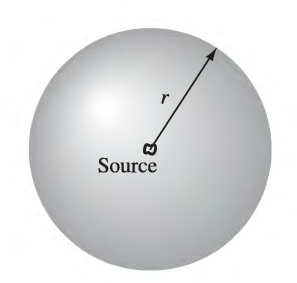
\includegraphics[width= 0.4\paperwidth, height= 0.07\paperheight]{1.png}
\end{center}
Well this is all pretty concrete, but what does it mean abstractly? A Group is simply a mathematical structure that follows a set of rules:
\begin{itemize}
\item $\forall \ a,b \in G: a \circ b \in G$
\item $\forall \ a,b,c \in G: a \circ (b \circ c) = (a \circ b) \circ c$	
\end{itemize}
\section{Rotation Groups}
The simplest example of a Group is present in rotations. This is also the easiest one to picture. So let's try to imagine a rotation in a two-dimensional plane (the Euclidian plane). We have a picture similar to this,
\begin{center}
	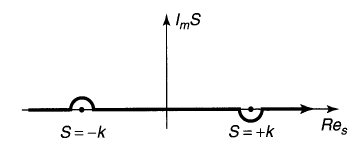
\includegraphics[width= 0.8\paperwidth, height= 0.8\paperheight]{2.png}
\end{center}
\subsection{Rotations in 3-dimensions}

\section{Lie Theory}
\subsection{Generators}
Any small transformation, for example a small rotation can be expressed as:
\begin{equation}
R(\theta) = I + \epsilon. g
\end{equation}
Where Epsilon is just a very small number and $g$ a matrix that expresses the transformation in a sense. Now, we can re-write $\epsilon$ as,
$$\epsilon = \frac{\theta}{N}$$
Thus, becomes:
\begin{equation}
R(\theta) = I + \epsilon. g
\end{equation}
How do we get to finite transformations? By repeatedly applying \ref{}. So we get something like:
\begin{equation}
R(\theta) = (I + \frac{\theta}{N}g)^{N}
\end{equation}
for $n$ transformations. Now if we consider it to be an infinitesimal transformation, we get:
\begin{equation}
R(\theta) = \lim\limits_{N \rightarrow \infty}(I + \frac{\theta}{N}g)^{N} = e^{g \theta}
\end{equation}
This is simply just the exponetial map. Here we call $g$, the \textbf{Generator} of rotations and $\theta$, the parameter. Why do we care about this you may ask?
\subsection{Lie Algebra}
Simply put, it's easier to deal with them for the following reasons:
\begin{itemize}
\item There are finite amount of Generators whereas infinite number of Group elements
\item All the elements of the Group can be built from the Generator itself
\item The elements of the Lie algebra form "neat" relationships
\end{itemize}

Formally speaking, the Lie algebras form a differentiable manifold that obey the following axioms:

\section{A Little Quantum Mechanics}
$$\ket{\psi}$$

This is known as a "Ket" or column vector. We can extract maximal information (i.e. as much as we can. This is not necessarily everything) about the system by applying operations to it, thus there is by nature an unpredictability about the future of the system. This is in stark contrast \href{https://arxiv.org/abs/1909.04514}{or maybe not} to classical physics, where knowing the state of something corresponds to knowing everything that can be known about it. The obvious question to ask is, "whether the unpredictability is due to an incompleteness in the a quantum state or is it due *hidden variables* that are inaccessible to us?". There are various opinions about this matter, this is still an \href{https://plato.stanford.edu/entries/qt-issues/#QuesQuanStatReal}{open issue}. However, for now we'll act as if there is an inherent unpredictability (despite newer theories having deterministic features) . This approach is called the "Copenhagen interpretation". We can also express the state vector as a superposition of other states\\

%$$⁍$$

Provided the complex numbers $\alpha$ and $\beta$, satisfy the condition

$$\alpha \alpha^{*} + \beta \beta^{*} = 1 $$

They are said to be normalized, we impose this condition because the complex conjugation represents the probability of something occurring and we want to ensure that all the probabilities add up to 1. Where the $*$ symbol represents complex conjugation. Similarly we can introduce a row vector called the "Bra", but however, since the elements are complex numbers we need to conjugate them as well

%$$⁍$$

*Where $T$ represents the transposition of a matrix and the $\dagger$ (dagger) represents complex conjugation followed by transpose.* 

*We can write it as,*

$$\langle \psi | \psi \rangle = \begin{pmatrix}
\psi^{*}_1 \ \psi^{*}_2
\end{pmatrix}\begin{pmatrix}
\psi_1 \\
\psi_2
\end{pmatrix}$$

$$\langle \psi | \psi \rangle = 
\psi_1 \psi^{*}_1 +  \psi_2\psi^{*}_2$$

This can still have negative numbers, so we take absolute value of it. However, this still doesn't represent probabilities since . Thus, we square it. This is analogous to finding the square of the length of the vector representing $\psi$,

$$|\langle \psi |\psi\rangle | ^{2} = 1$$

This is called the ***"Born rule"***, as it was first suggested by Max Born.

\subsection{Observables}

We can apply operations to the state vector to find out what happens to measurable quantities such as momentum and position. The operations are termed as \textbf{operators} and are represented using matrices

$$\hat{O} = \begin{pmatrix}
O_{11} & O_{12}\\
O_{21} & O_{22}
\end{pmatrix}$$
These operators are termed linear that is they follow the properties:
$$(\hat{O}_1 + \hat{O}_2)|\psi\rangle = \hat{O}_1|\psi\rangle+ \hat{O}_2 |\psi\rangle$$
$$\hat{O} (\alpha |\psi\rangle) = \alpha \hat{O} |\psi\rangle$$
$\forall \ \alpha \in \mathbb{C}$

For example the momentum operator is given by the equation
$$\hat{P} = -i \hbar \frac{\partial}{\partial x}$$
where $i$ is the imaginary number, $\hbar = \frac{h}{2 \pi}$ a physical constant. So if we look at how it operates it is easy to see that

$$\hat{P}|\psi\rangle = -i \hbar \frac{\partial | \psi \rangle}{\partial x}$$

\subsection{Math interlude: Matrices}

\subsubsection{Matrix Multiplication}

When we multiply two number A and B for instance, we have this property
$$AB = BA$$
this is called as commutativity. However, when deal with operators we're dealing with matrices, so in general
$$\hat{A}\hat{B} \neq \hat{B}\hat{A}$$
But in a few cases two operators can commute, thus we use a measure called the *"Commutator"* to quantify if or not two operators commute
$$[\hat{A}, \hat{B}] = \hat{A}\hat{B} - \hat{B}\hat{A}$$
Thus, if the commutator is 0 then the operators commute, if not then they don't commute. As the commutator can only be zero if the condition Eq.(1) is satisfied.\footnote{SPOILER: We shall find that if two operators commute then it is possible to measure them both simultaneously}

Moreover we can represent the multiplication of a Bra and a Ket as\footnote{This is quite analogous to the dot product operation},
$$\langle X|Y \rangle = \langle X | \  |Y\rangle = \begin{pmatrix}
x_1 \ x_2
\end{pmatrix} \begin{pmatrix}
y_1 \\
y_2
\end{pmatrix}$$
and it is quite easy to see that
$\langle X | X \rangle = |X|^2$

\subsection{Eigen-stuff}

Since operators are basically matrices, we can also have the "transformation" picture in mind. That is, when I multiply a vector or in this case the state vector with a matrix I make a change to it. EXPAND

Most of the time the , but there are a few vectors such that their direction remains unchanged, they are called ***Eigenvectors***. Their direction isn't changed however there is no constraint on how the length is changed, so sometimes their length is scaled up or down by multiplying it with a real number called an ***Eigenvalue***. 

%[]()

That is in summary, the effect the operator has on that particular vector is equal to multiplying it by a real number.

%$$⁍$$

What does this mean for Quantum Mechanics? Each Eigenvalue represents something that can be measured by applying that operator. More importantly, this will always be a real number as we can only measure real numbers. For more dig deep into Eigen-stuff head to [article promo text](https://elliptigon.com/eigendecomposition/).

\section{Spin}
One may ask what is spin but not why spin? To answer this question in a physical sense, spin is simply the internal angular monetum of a quantum mechanical object. It is yet another entity in quantum mechanics that does not have a classical analog. What do we know of it? We know for a fact that it is discete. That is when you act with the spin operator on a 
However, $s$ can in fact be a "half-integer" as well as an integer, which is to say:
$$s = 0, \frac{1}{2}, 1, \frac{3}{2}, 2, \frac{5}{2}, 3, ...$$

\section{A Deeper Look at $SU(2)$}

\subsection{Addition of Angular Momenta}
Another interesting question that we can pose is, how do we add Angular momenta? 
\subsection{Spin $\frac{1}{2}$}

\section{A Little More Lie Theory}
Irreps are the smallest set of states of a representation of a given dimension that is closed under the action of the symmetry group. A Casimir is defined as the sum of the operators squared in a particular representation. For example, let's look at Spin:
\begin{equation}
\hat{S}^{2} = \hat{S}_{x}^{2}
\end{equation}
It is rotation invariant and measures the magnitude of spin

\section{A Short tale about Quarks}
It all begins in Heisenberg's Hypothesis that based on this data,
he suggested that there must exist an approximate symmetry called Isospin between protons and neutrons. Let's try to see how this works, first lets consider the state vectors for a neutron and for a proton with the following properties.
\begin{equation}
\braket{n}{n} = \braket{p}{p} = 1
\end{equation}
\begin{equation}
\braket{p}{n} = \braket{n}{p} = 0
\end{equation}
In a sesnse symmetry between protons and neutrons means that any linear combination i.e. superpositions of their wavefunctions describes the same physics. We'll call this generic combination the nucleon state, denoted by:
\begin{equation}
\ket{N} = \alpha \ket{p} +  \beta \ket{n}
\end{equation}
where, $\alpha, \beta \in \mathbb{C}$ and $\abs{\alpha}^{2} + \abs{\beta}^{2} = 1 = \braket{N}{N}$
Correspondingly, the proton and neutron transform as a two-dimensional representation of isospin, appropriately referred to as an isospin doublet. Higher-dimensional representations of these groups exist, but they have the property that they can be formed from the smallest dimensional representation. As such, the smallest-dimensional representation of a group is called the fundamental representation.
In this universe where there is an exact SU(2) isospin symmetry between protons and neutrons, Noether’s theorem tells us that in reactions involving protons and neutrons, isospin is conserved. Of course, this isn’t our universe, but in processes where the differences between protons and neutrons are irrelevant (or not dominant), we do expect isospin conservation. In particular,
as long as we study protons and neutrons in a way that doesn’t involve electromagnetism or don’t care about the neutron decay, then isospin should be conserved. And this what we see happening. Essentially what we've done so far is construct an internal space called Isospin for every point in spacetime and argue that it be invariant under representations of a particular group. This representation is the 
\section*{References}
\begin{itemize}
\item Alex Flournoy's Lectures on Particle Physics, 2016
\item A Child’s Guide to Spinors by William O. Straub
\item arXiv:1312.3824 [math-ph], An introduction to spinors by Andrew M. Steane 
\item Carter, N. (2009). Visual Group Theory. Cambridge Univ Pr.
\item Stillwell, J. (2012). Naive lie theory. Beijing: World Publishing Corporation.
\item Griffiths, D. J. (2005). Introduction to quantum mechanics. Upper Saddle River, NJ: Pearson/Prentice Hall.
\item Shankar, R. (1994). Principles of quantum mechanics. New York: Springer.
\item Artin, M. (2018). Algebra. NY, NY: Pearson.
\item Schwichtenberg, J. (2018). Physics from symmetry. Cham, Switzerland: Springer.
\item Griffiths, D. J. (2014). Introduction to elementary particles. Weinheim: Wiley-VCH Verlag.
\item Larkoski, A. J. (2019). Elementary particle physics: An intuitive introduction. Cambridge, United Kingdom: Cambridge University Press.
\end{itemize}
\end{document}
